% !TeX spellcheck = en_GB
\subsection{The automatic index updating feature}

\subsubsection{Overview of possible implementations}

\paragraph{Synchronous approaches}

\subparagraph{JPA events}

\subparagraph{Native integrations with JPA providers}

\paragraph{Asynchronous Trigger approach}
~\\



\subsubsection{Implementation details}

\paragraph{Native events}
~\\

\paragraph{Triggers}
~\\

includeEmbeddedObjectId = true ist Pflicht!

\lstset{language=java}
\lstset{moredelim=[is][\bfseries]{[*}{*]}}
\begin{lstlisting}[frame=htrbl, caption={Book.java with Hibernate Search annotations}, label={lst:book.java_3}]
@Entity
@InIndex
@Table(name = "Book")
@Indexed
[*@UpdateInfo(
	tableName = "Book", 
	idInfos = 
	@IdInfo(columns = 
		@IdColumn(
			column = "isbn", 
			columnType = ColumnType.STRING
		)
	)
)*]
public class Book {

	// ... unchanged. 
	
	//mapping table events handled on Author side
	
	//getters & setters ...
}
\end{lstlisting}

\lstset{language=java}
\lstset{moredelim=[is][\bfseries]{[*}{*]}}
\begin{lstlisting}[frame=htrbl, caption={Author.java with Hibernate Search annotations}, label={lst:author.java_3}]
@Entity
@InIndex
@Table(name = "Author")
[*@UpdateInfo(
	tableName = "Author", 
	idInfos = 
	@IdInfo(columns = 
		@IdColumn(
			column = "authorId", 
			columnType = ColumnType.LONG
		)
	)
)*]
public class Author {
	
	// ... unchanged.
	
	[*@UpdateInfo(tableName = "Author_Book", 
		idInfos = {
		@IdInfo(entity = Author.class, 
			columns = 
			@IdColumn(
				column = "authorFk",
				columnType = ColumnType.LONG
			)
		),
		@IdInfo(entity = Book.class,
			columns = 
			@IdColumn(
				column = "bookFk",
				columnType = ColumnType.STRING
			)
		)
	})*]
	private Set<Book> books;
	
	//getters & setters ...
}
\end{lstlisting}

\begin{figure}[ht]
	\centering
	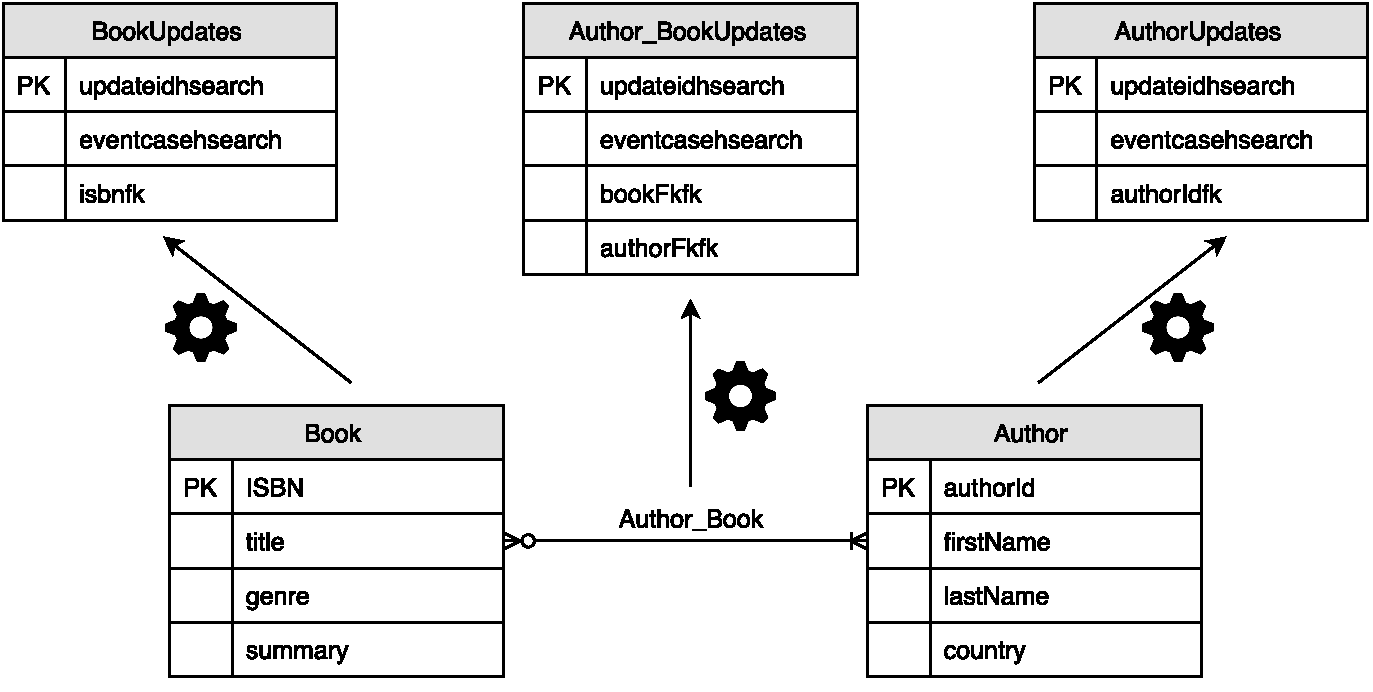
\includegraphics[scale=0.6]{images/Triggers_Schema.pdf}
	\caption{Triggers for the example project}
	\label{triggers_schema}
\end{figure}

\subsubsection{Complete Update System overview}

\begin{figure}[ht]
	\centering
	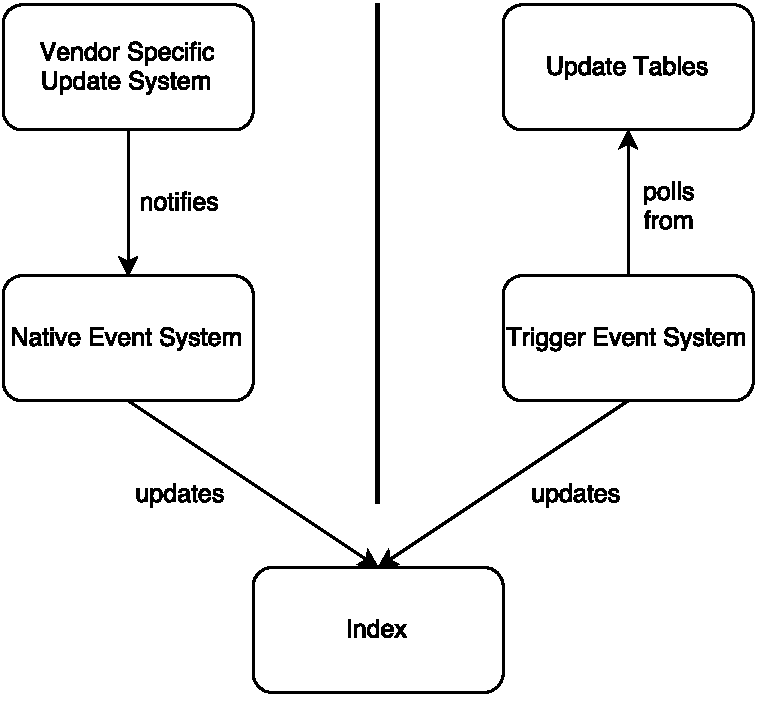
\includegraphics[scale=0.6]{images/UpdateConsumer_Architecture.pdf}
	\caption{Triggers for the example project}
	\label{updateconsumer_architecture}
\end{figure}

\pagebreak